% Created by tikzDevice version 0.12.3.1 on 2021-05-24 14:07:42
% !TEX encoding = UTF-8 Unicode
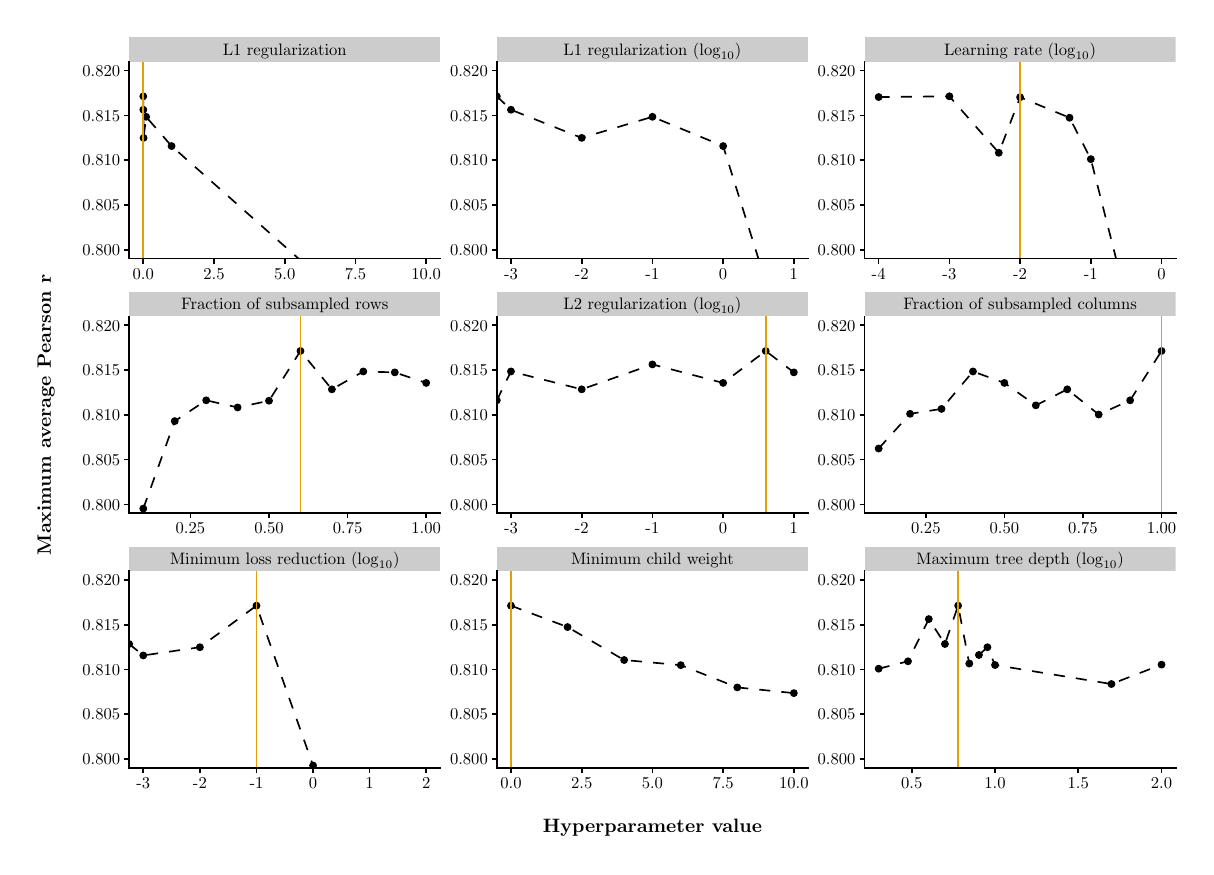
\begin{tikzpicture}[x=1pt,y=1pt]
	\definecolor{fillColor}{RGB}{255,255,255}
	\path[use as bounding box,fill=fillColor,fill opacity=0.00] (0,0) rectangle (418.34,295.82);
	\begin{scope}
		\path[clip] ( 36.67,212.35) rectangle (149.11,283.52);
		\definecolor{drawColor}{RGB}{0,0,0}
		\definecolor{fillColor}{RGB}{0,0,0}

		\path[draw=drawColor,line width= 0.4pt,line join=round,line cap=round,fill=fillColor] ( 41.78,271.01) circle (  1.21);

		\path[draw=drawColor,line width= 0.4pt,line join=round,line cap=round,fill=fillColor] ( 41.79,266.16) circle (  1.21);

		\path[draw=drawColor,line width= 0.4pt,line join=round,line cap=round,fill=fillColor] ( 41.88,255.99) circle (  1.21);

		\path[draw=drawColor,line width= 0.4pt,line join=round,line cap=round,fill=fillColor] ( 42.80,263.61) circle (  1.21);

		\path[draw=drawColor,line width= 0.4pt,line join=round,line cap=round,fill=fillColor] ( 52.00,253.03) circle (  1.21);

		\path[draw=drawColor,line width= 0.4pt,line join=round,line cap=round,fill=fillColor] (144.00,171.49) circle (  1.21);

		\path[draw=drawColor,line width= 0.6pt,dash pattern=on 4pt off 4pt ,line join=round] ( 41.78,271.01) --
		( 41.79,266.16) --
		( 41.88,255.99) --
		( 42.80,263.61) --
		( 52.00,253.03) --
		(144.00,171.49);
		\definecolor{drawColor}{RGB}{230,159,0}

		\path[draw=drawColor,line width= 0.6pt,line join=round] ( 41.78,212.35) -- ( 41.78,283.52);
	\end{scope}
	\begin{scope}
		\path[clip] ( 36.67,120.33) rectangle (149.11,191.50);
		\definecolor{drawColor}{RGB}{0,0,0}
		\definecolor{fillColor}{RGB}{0,0,0}

		\path[draw=drawColor,line width= 0.4pt,line join=round,line cap=round,fill=fillColor] ( 41.78,122.04) circle (  1.21);

		\path[draw=drawColor,line width= 0.4pt,line join=round,line cap=round,fill=fillColor] ( 53.14,153.65) circle (  1.21);

		\path[draw=drawColor,line width= 0.4pt,line join=round,line cap=round,fill=fillColor] ( 64.50,161.16) circle (  1.21);

		\path[draw=drawColor,line width= 0.4pt,line join=round,line cap=round,fill=fillColor] ( 75.86,158.59) circle (  1.21);

		\path[draw=drawColor,line width= 0.4pt,line join=round,line cap=round,fill=fillColor] ( 87.21,161.01) circle (  1.21);

		\path[draw=drawColor,line width= 0.4pt,line join=round,line cap=round,fill=fillColor] ( 98.57,178.99) circle (  1.21);

		\path[draw=drawColor,line width= 0.4pt,line join=round,line cap=round,fill=fillColor] (109.93,165.13) circle (  1.21);

		\path[draw=drawColor,line width= 0.4pt,line join=round,line cap=round,fill=fillColor] (121.29,171.59) circle (  1.21);

		\path[draw=drawColor,line width= 0.4pt,line join=round,line cap=round,fill=fillColor] (132.65,171.26) circle (  1.21);

		\path[draw=drawColor,line width= 0.4pt,line join=round,line cap=round,fill=fillColor] (144.00,167.45) circle (  1.21);

		\path[draw=drawColor,line width= 0.6pt,dash pattern=on 4pt off 4pt ,line join=round] ( 41.78,122.04) --
		( 53.14,153.65) --
		( 64.50,161.16) --
		( 75.86,158.59) --
		( 87.21,161.01) --
		( 98.57,178.99) --
		(109.93,165.13) --
		(121.29,171.59) --
		(132.65,171.26) --
		(144.00,167.45);
		\definecolor{drawColor}{RGB}{230,159,0}

		\path[draw=drawColor,line width= 0.6pt,line join=round] ( 98.57,120.33) -- ( 98.57,191.50);
	\end{scope}
	\begin{scope}
		\path[clip] ( 36.67, 28.30) rectangle (149.11, 99.48);
		\definecolor{drawColor}{RGB}{0,0,0}
		\definecolor{fillColor}{RGB}{0,0,0}

		\path[draw=drawColor,line width= 0.4pt,line join=round,line cap=round,fill=fillColor] ( 36.67, 73.11) circle (  1.21);

		\path[draw=drawColor,line width= 0.4pt,line join=round,line cap=round,fill=fillColor] ( 41.78, 68.98) circle (  1.21);

		\path[draw=drawColor,line width= 0.4pt,line join=round,line cap=round,fill=fillColor] ( 62.23, 71.94) circle (  1.21);

		\path[draw=drawColor,line width= 0.4pt,line join=round,line cap=round,fill=fillColor] ( 82.67, 86.97) circle (  1.21);

		\path[draw=drawColor,line width= 0.4pt,line join=round,line cap=round,fill=fillColor] (103.12, 29.20) circle (  1.21);

		\path[draw=drawColor,line width= 0.4pt,line join=round,line cap=round,fill=fillColor] (123.56,-433.02) circle (  1.21);

		\path[draw=drawColor,line width= 0.4pt,line join=round,line cap=round,fill=fillColor] (144.00,-1376.23) circle (  1.21);

		\path[draw=drawColor,line width= 0.6pt,dash pattern=on 4pt off 4pt ,line join=round] ( 36.67, 73.11) --
		( 41.78, 68.98) --
		( 62.23, 71.94) --
		( 82.67, 86.97) --
		(103.12, 29.20) --
		(123.56,-433.02) --
		(144.00,-1376.23);
		\definecolor{drawColor}{RGB}{230,159,0}

		\path[draw=drawColor,line width= 0.6pt,line join=round] ( 82.67, 28.30) -- ( 82.67, 99.48);
	\end{scope}
	\begin{scope}
		\path[clip] (169.53,212.35) rectangle (281.98,283.52);
		\definecolor{drawColor}{RGB}{0,0,0}
		\definecolor{fillColor}{RGB}{0,0,0}

		\path[draw=drawColor,line width= 0.4pt,line join=round,line cap=round,fill=fillColor] (169.53,271.01) circle (  1.21);

		\path[draw=drawColor,line width= 0.4pt,line join=round,line cap=round,fill=fillColor] (174.64,266.16) circle (  1.21);

		\path[draw=drawColor,line width= 0.4pt,line join=round,line cap=round,fill=fillColor] (200.20,255.99) circle (  1.21);

		\path[draw=drawColor,line width= 0.4pt,line join=round,line cap=round,fill=fillColor] (225.75,263.61) circle (  1.21);

		\path[draw=drawColor,line width= 0.4pt,line join=round,line cap=round,fill=fillColor] (251.31,253.03) circle (  1.21);

		\path[draw=drawColor,line width= 0.4pt,line join=round,line cap=round,fill=fillColor] (276.86,171.49) circle (  1.21);

		\path[draw=drawColor,line width= 0.6pt,dash pattern=on 4pt off 4pt ,line join=round] (169.53,271.01) --
		(174.64,266.16) --
		(200.20,255.99) --
		(225.75,263.61) --
		(251.31,253.03) --
		(276.86,171.49);
		\definecolor{drawColor}{RGB}{230,159,0}

		\path[draw=drawColor,line width= 0.6pt,line join=round] (169.53,212.35) -- (169.53,283.52);
	\end{scope}
	\begin{scope}
		\path[clip] (169.53,120.33) rectangle (281.98,191.50);
		\definecolor{drawColor}{RGB}{0,0,0}
		\definecolor{fillColor}{RGB}{0,0,0}

		\path[draw=drawColor,line width= 0.4pt,line join=round,line cap=round,fill=fillColor] (169.53,161.16) circle (  1.21);

		\path[draw=drawColor,line width= 0.4pt,line join=round,line cap=round,fill=fillColor] (174.64,171.59) circle (  1.21);

		\path[draw=drawColor,line width= 0.4pt,line join=round,line cap=round,fill=fillColor] (200.20,165.13) circle (  1.21);

		\path[draw=drawColor,line width= 0.4pt,line join=round,line cap=round,fill=fillColor] (225.75,174.13) circle (  1.21);

		\path[draw=drawColor,line width= 0.4pt,line join=round,line cap=round,fill=fillColor] (251.31,167.45) circle (  1.21);

		\path[draw=drawColor,line width= 0.4pt,line join=round,line cap=round,fill=fillColor] (266.69,178.99) circle (  1.21);

		\path[draw=drawColor,line width= 0.4pt,line join=round,line cap=round,fill=fillColor] (276.86,171.26) circle (  1.21);

		\path[draw=drawColor,line width= 0.6pt,dash pattern=on 4pt off 4pt ,line join=round] (169.53,161.16) --
		(174.64,171.59) --
		(200.20,165.13) --
		(225.75,174.13) --
		(251.31,167.45) --
		(266.69,178.99) --
		(276.86,171.26);
		\definecolor{drawColor}{RGB}{230,159,0}

		\path[draw=drawColor,line width= 0.6pt,line join=round] (266.69,120.33) -- (266.69,191.50);
	\end{scope}
	\begin{scope}
		\path[clip] (169.53, 28.30) rectangle (281.98, 99.48);
		\definecolor{drawColor}{RGB}{0,0,0}
		\definecolor{fillColor}{RGB}{0,0,0}

		\path[draw=drawColor,line width= 0.4pt,line join=round,line cap=round,fill=fillColor] (174.64, 86.97) circle (  1.21);

		\path[draw=drawColor,line width= 0.4pt,line join=round,line cap=round,fill=fillColor] (195.09, 79.23) circle (  1.21);

		\path[draw=drawColor,line width= 0.4pt,line join=round,line cap=round,fill=fillColor] (215.53, 67.32) circle (  1.21);

		\path[draw=drawColor,line width= 0.4pt,line join=round,line cap=round,fill=fillColor] (235.98, 65.47) circle (  1.21);

		\path[draw=drawColor,line width= 0.4pt,line join=round,line cap=round,fill=fillColor] (256.42, 57.42) circle (  1.21);

		\path[draw=drawColor,line width= 0.4pt,line join=round,line cap=round,fill=fillColor] (276.86, 55.36) circle (  1.21);

		\path[draw=drawColor,line width= 0.6pt,dash pattern=on 4pt off 4pt ,line join=round] (174.64, 86.97) --
		(195.09, 79.23) --
		(215.53, 67.32) --
		(235.98, 65.47) --
		(256.42, 57.42) --
		(276.86, 55.36);
		\definecolor{drawColor}{RGB}{230,159,0}

		\path[draw=drawColor,line width= 0.6pt,line join=round] (174.64, 28.30) -- (174.64, 99.48);
	\end{scope}
	\begin{scope}
		\path[clip] (302.39,212.35) rectangle (414.84,283.52);
		\definecolor{drawColor}{RGB}{0,0,0}
		\definecolor{fillColor}{RGB}{0,0,0}

		\path[draw=drawColor,line width= 0.4pt,line join=round,line cap=round,fill=fillColor] (307.50,270.75) circle (  1.21);

		\path[draw=drawColor,line width= 0.4pt,line join=round,line cap=round,fill=fillColor] (333.06,271.01) circle (  1.21);

		\path[draw=drawColor,line width= 0.4pt,line join=round,line cap=round,fill=fillColor] (350.92,250.61) circle (  1.21);

		\path[draw=drawColor,line width= 0.4pt,line join=round,line cap=round,fill=fillColor] (358.61,270.68) circle (  1.21);

		\path[draw=drawColor,line width= 0.4pt,line join=round,line cap=round,fill=fillColor] (376.48,263.28) circle (  1.21);

		\path[draw=drawColor,line width= 0.4pt,line join=round,line cap=round,fill=fillColor] (384.17,248.31) circle (  1.21);

		\path[draw=drawColor,line width= 0.4pt,line join=round,line cap=round,fill=fillColor] (402.03,177.91) circle (  1.21);

		\path[draw=drawColor,line width= 0.4pt,line join=round,line cap=round,fill=fillColor] (409.72,-98.71) circle (  1.21);

		\path[draw=drawColor,line width= 0.6pt,dash pattern=on 4pt off 4pt ,line join=round] (307.50,270.75) --
		(333.06,271.01) --
		(350.92,250.61) --
		(358.61,270.68) --
		(376.48,263.28) --
		(384.17,248.31) --
		(402.03,177.91) --
		(409.72,-98.71);
		\definecolor{drawColor}{RGB}{230,159,0}

		\path[draw=drawColor,line width= 0.6pt,line join=round] (358.61,212.35) -- (358.61,283.52);
	\end{scope}
	\begin{scope}
		\path[clip] (302.39,120.33) rectangle (414.84,191.50);
		\definecolor{drawColor}{RGB}{0,0,0}
		\definecolor{fillColor}{RGB}{0,0,0}

		\path[draw=drawColor,line width= 0.4pt,line join=round,line cap=round,fill=fillColor] (307.50,143.75) circle (  1.21);

		\path[draw=drawColor,line width= 0.4pt,line join=round,line cap=round,fill=fillColor] (318.86,156.29) circle (  1.21);

		\path[draw=drawColor,line width= 0.4pt,line join=round,line cap=round,fill=fillColor] (330.22,158.06) circle (  1.21);

		\path[draw=drawColor,line width= 0.4pt,line join=round,line cap=round,fill=fillColor] (341.58,171.59) circle (  1.21);

		\path[draw=drawColor,line width= 0.4pt,line join=round,line cap=round,fill=fillColor] (352.93,167.45) circle (  1.21);

		\path[draw=drawColor,line width= 0.4pt,line join=round,line cap=round,fill=fillColor] (364.29,159.34) circle (  1.21);

		\path[draw=drawColor,line width= 0.4pt,line join=round,line cap=round,fill=fillColor] (375.65,165.13) circle (  1.21);

		\path[draw=drawColor,line width= 0.4pt,line join=round,line cap=round,fill=fillColor] (387.01,156.03) circle (  1.21);

		\path[draw=drawColor,line width= 0.4pt,line join=round,line cap=round,fill=fillColor] (398.37,161.16) circle (  1.21);

		\path[draw=drawColor,line width= 0.4pt,line join=round,line cap=round,fill=fillColor] (409.72,178.99) circle (  1.21);

		\path[draw=drawColor,line width= 0.6pt,dash pattern=on 4pt off 4pt ,line join=round] (307.50,143.75) --
		(318.86,156.29) --
		(330.22,158.06) --
		(341.58,171.59) --
		(352.93,167.45) --
		(364.29,159.34) --
		(375.65,165.13) --
		(387.01,156.03) --
		(398.37,161.16) --
		(409.72,178.99);
		\definecolor{drawColor}{RGB}{230,159,0}

		\path[draw=drawColor,line width= 0.6pt,line join=round] (409.72,120.33) -- (409.72,191.50);
	\end{scope}
	\begin{scope}
		\path[clip] (302.39, 28.30) rectangle (414.84, 99.48);
		\definecolor{drawColor}{RGB}{0,0,0}
		\definecolor{fillColor}{RGB}{0,0,0}

		\path[draw=drawColor,line width= 0.4pt,line join=round,line cap=round,fill=fillColor] (307.50, 64.19) circle (  1.21);

		\path[draw=drawColor,line width= 0.4pt,line join=round,line cap=round,fill=fillColor] (318.10, 66.86) circle (  1.21);

		\path[draw=drawColor,line width= 0.4pt,line join=round,line cap=round,fill=fillColor] (325.62, 82.11) circle (  1.21);

		\path[draw=drawColor,line width= 0.4pt,line join=round,line cap=round,fill=fillColor] (331.45, 73.11) circle (  1.21);

		\path[draw=drawColor,line width= 0.4pt,line join=round,line cap=round,fill=fillColor] (336.21, 86.97) circle (  1.21);

		\path[draw=drawColor,line width= 0.4pt,line join=round,line cap=round,fill=fillColor] (340.24, 66.03) circle (  1.21);

		\path[draw=drawColor,line width= 0.4pt,line join=round,line cap=round,fill=fillColor] (343.73, 69.14) circle (  1.21);

		\path[draw=drawColor,line width= 0.4pt,line join=round,line cap=round,fill=fillColor] (346.80, 71.94) circle (  1.21);

		\path[draw=drawColor,line width= 0.4pt,line join=round,line cap=round,fill=fillColor] (349.56, 65.51) circle (  1.21);

		\path[draw=drawColor,line width= 0.4pt,line join=round,line cap=round,fill=fillColor] (391.61, 58.65) circle (  1.21);

		\path[draw=drawColor,line width= 0.4pt,line join=round,line cap=round,fill=fillColor] (409.72, 65.66) circle (  1.21);

		\path[draw=drawColor,line width= 0.6pt,dash pattern=on 4pt off 4pt ,line join=round] (307.50, 64.19) --
		(318.10, 66.86) --
		(325.62, 82.11) --
		(331.45, 73.11) --
		(336.21, 86.97) --
		(340.24, 66.03) --
		(343.73, 69.14) --
		(346.80, 71.94) --
		(349.56, 65.51) --
		(391.61, 58.65) --
		(409.72, 65.66);
		\definecolor{drawColor}{RGB}{230,159,0}

		\path[draw=drawColor,line width= 0.6pt,line join=round] (336.21, 28.30) -- (336.21, 99.48);
	\end{scope}
	\begin{scope}
		\path[clip] ( 36.67, 99.48) rectangle (149.11,108.28);
		\definecolor{fillColor}{gray}{0.80}

		\path[fill=fillColor] ( 36.67, 99.48) rectangle (149.11,108.28);
		\definecolor{drawColor}{RGB}{0,0,0}

		\node[text=drawColor,anchor=base,inner sep=0pt, outer sep=0pt, scale=  0.60] at ( 92.89,101.81) {Minimum loss reduction ($\log_{10}$)};
	\end{scope}
	\begin{scope}
		\path[clip] (169.53, 99.48) rectangle (281.98,108.28);
		\definecolor{fillColor}{gray}{0.80}

		\path[fill=fillColor] (169.53, 99.48) rectangle (281.98,108.28);
		\definecolor{drawColor}{RGB}{0,0,0}

		\node[text=drawColor,anchor=base,inner sep=0pt, outer sep=0pt, scale=  0.60] at (225.75,101.81) {Minimum child weight};
	\end{scope}
	\begin{scope}
		\path[clip] (302.39, 99.48) rectangle (414.84,108.28);
		\definecolor{fillColor}{gray}{0.80}

		\path[fill=fillColor] (302.39, 99.48) rectangle (414.84,108.28);
		\definecolor{drawColor}{RGB}{0,0,0}

		\node[text=drawColor,anchor=base,inner sep=0pt, outer sep=0pt, scale=  0.60] at (358.61,101.81) {Maximum tree depth ($\log_{10}$)};
	\end{scope}
	\begin{scope}
		\path[clip] ( 36.67,191.50) rectangle (149.11,200.30);
		\definecolor{fillColor}{gray}{0.80}

		\path[fill=fillColor] ( 36.67,191.50) rectangle (149.11,200.30);
		\definecolor{drawColor}{RGB}{0,0,0}

		\node[text=drawColor,anchor=base,inner sep=0pt, outer sep=0pt, scale=  0.60] at ( 92.89,193.83) {Fraction of subsampled rows};
	\end{scope}
	\begin{scope}
		\path[clip] (169.53,191.50) rectangle (281.98,200.30);
		\definecolor{fillColor}{gray}{0.80}

		\path[fill=fillColor] (169.53,191.50) rectangle (281.98,200.30);
		\definecolor{drawColor}{RGB}{0,0,0}

		\node[text=drawColor,anchor=base,inner sep=0pt, outer sep=0pt, scale=  0.60] at (225.75,193.83) {L2 regularization ($\log_{10}$)};
	\end{scope}
	\begin{scope}
		\path[clip] (302.39,191.50) rectangle (414.84,200.30);
		\definecolor{fillColor}{gray}{0.80}

		\path[fill=fillColor] (302.39,191.50) rectangle (414.84,200.30);
		\definecolor{drawColor}{RGB}{0,0,0}

		\node[text=drawColor,anchor=base,inner sep=0pt, outer sep=0pt, scale=  0.60] at (358.61,193.83) {Fraction of subsampled columns};
	\end{scope}
	\begin{scope}
		\path[clip] ( 36.67,283.52) rectangle (149.11,292.32);
		\definecolor{fillColor}{gray}{0.80}

		\path[fill=fillColor] ( 36.67,283.52) rectangle (149.11,292.32);
		\definecolor{drawColor}{RGB}{0,0,0}

		\node[text=drawColor,anchor=base,inner sep=0pt, outer sep=0pt, scale=  0.60] at ( 92.89,285.86) {L1 regularization};
	\end{scope}
	\begin{scope}
		\path[clip] (169.53,283.52) rectangle (281.98,292.32);
		\definecolor{fillColor}{gray}{0.80}

		\path[fill=fillColor] (169.53,283.52) rectangle (281.98,292.32);
		\definecolor{drawColor}{RGB}{0,0,0}

		\node[text=drawColor,anchor=base,inner sep=0pt, outer sep=0pt, scale=  0.60] at (225.75,285.86) {L1 regularization ($\log_{10}$)};
	\end{scope}
	\begin{scope}
		\path[clip] (302.39,283.52) rectangle (414.84,292.32);
		\definecolor{fillColor}{gray}{0.80}

		\path[fill=fillColor] (302.39,283.52) rectangle (414.84,292.32);
		\definecolor{drawColor}{RGB}{0,0,0}

		\node[text=drawColor,anchor=base,inner sep=0pt, outer sep=0pt, scale=  0.60] at (358.61,285.86) {Learning rate ($\log_{10}$)};
	\end{scope}
	\begin{scope}
		\path[clip] (  0.00,  0.00) rectangle (418.34,295.82);
		\definecolor{drawColor}{RGB}{0,0,0}

		\path[draw=drawColor,line width= 0.6pt,line join=round,line cap=rect] ( 36.67, 28.30) --
		(149.11, 28.30);
	\end{scope}
	\begin{scope}
		\path[clip] (  0.00,  0.00) rectangle (418.34,295.82);
		\definecolor{drawColor}{RGB}{0,0,0}

		\path[draw=drawColor,line width= 0.6pt,line join=round] ( 41.78, 26.55) --
		( 41.78, 28.30);

		\path[draw=drawColor,line width= 0.6pt,line join=round] ( 62.23, 26.55) --
		( 62.23, 28.30);

		\path[draw=drawColor,line width= 0.6pt,line join=round] ( 82.67, 26.55) --
		( 82.67, 28.30);

		\path[draw=drawColor,line width= 0.6pt,line join=round] (103.12, 26.55) --
		(103.12, 28.30);

		\path[draw=drawColor,line width= 0.6pt,line join=round] (123.56, 26.55) --
		(123.56, 28.30);

		\path[draw=drawColor,line width= 0.6pt,line join=round] (144.00, 26.55) --
		(144.00, 28.30);
	\end{scope}
	\begin{scope}
		\path[clip] (  0.00,  0.00) rectangle (418.34,295.82);
		\definecolor{drawColor}{RGB}{0,0,0}

		\node[text=drawColor,anchor=base,inner sep=0pt, outer sep=0pt, scale=  0.60] at ( 41.78, 20.92) {-3};

		\node[text=drawColor,anchor=base,inner sep=0pt, outer sep=0pt, scale=  0.60] at ( 62.23, 20.92) {-2};

		\node[text=drawColor,anchor=base,inner sep=0pt, outer sep=0pt, scale=  0.60] at ( 82.67, 20.92) {-1};

		\node[text=drawColor,anchor=base,inner sep=0pt, outer sep=0pt, scale=  0.60] at (103.12, 20.92) {0};

		\node[text=drawColor,anchor=base,inner sep=0pt, outer sep=0pt, scale=  0.60] at (123.56, 20.92) {1};

		\node[text=drawColor,anchor=base,inner sep=0pt, outer sep=0pt, scale=  0.60] at (144.00, 20.92) {2};
	\end{scope}
	\begin{scope}
		\path[clip] (  0.00,  0.00) rectangle (418.34,295.82);
		\definecolor{drawColor}{RGB}{0,0,0}

		\path[draw=drawColor,line width= 0.6pt,line join=round,line cap=rect] (169.53, 28.30) --
		(281.98, 28.30);
	\end{scope}
	\begin{scope}
		\path[clip] (  0.00,  0.00) rectangle (418.34,295.82);
		\definecolor{drawColor}{RGB}{0,0,0}

		\path[draw=drawColor,line width= 0.6pt,line join=round] (174.64, 26.55) --
		(174.64, 28.30);

		\path[draw=drawColor,line width= 0.6pt,line join=round] (200.20, 26.55) --
		(200.20, 28.30);

		\path[draw=drawColor,line width= 0.6pt,line join=round] (225.75, 26.55) --
		(225.75, 28.30);

		\path[draw=drawColor,line width= 0.6pt,line join=round] (251.31, 26.55) --
		(251.31, 28.30);

		\path[draw=drawColor,line width= 0.6pt,line join=round] (276.86, 26.55) --
		(276.86, 28.30);
	\end{scope}
	\begin{scope}
		\path[clip] (  0.00,  0.00) rectangle (418.34,295.82);
		\definecolor{drawColor}{RGB}{0,0,0}

		\node[text=drawColor,anchor=base,inner sep=0pt, outer sep=0pt, scale=  0.60] at (174.64, 20.92) {0.0};

		\node[text=drawColor,anchor=base,inner sep=0pt, outer sep=0pt, scale=  0.60] at (200.20, 20.92) {2.5};

		\node[text=drawColor,anchor=base,inner sep=0pt, outer sep=0pt, scale=  0.60] at (225.75, 20.92) {5.0};

		\node[text=drawColor,anchor=base,inner sep=0pt, outer sep=0pt, scale=  0.60] at (251.31, 20.92) {7.5};

		\node[text=drawColor,anchor=base,inner sep=0pt, outer sep=0pt, scale=  0.60] at (276.86, 20.92) {10.0};
	\end{scope}
	\begin{scope}
		\path[clip] (  0.00,  0.00) rectangle (418.34,295.82);
		\definecolor{drawColor}{RGB}{0,0,0}

		\path[draw=drawColor,line width= 0.6pt,line join=round,line cap=rect] (302.39, 28.30) --
		(414.84, 28.30);
	\end{scope}
	\begin{scope}
		\path[clip] (  0.00,  0.00) rectangle (418.34,295.82);
		\definecolor{drawColor}{RGB}{0,0,0}

		\path[draw=drawColor,line width= 0.6pt,line join=round] (319.47, 26.55) --
		(319.47, 28.30);

		\path[draw=drawColor,line width= 0.6pt,line join=round] (349.56, 26.55) --
		(349.56, 28.30);

		\path[draw=drawColor,line width= 0.6pt,line join=round] (379.64, 26.55) --
		(379.64, 28.30);

		\path[draw=drawColor,line width= 0.6pt,line join=round] (409.72, 26.55) --
		(409.72, 28.30);
	\end{scope}
	\begin{scope}
		\path[clip] (  0.00,  0.00) rectangle (418.34,295.82);
		\definecolor{drawColor}{RGB}{0,0,0}

		\node[text=drawColor,anchor=base,inner sep=0pt, outer sep=0pt, scale=  0.60] at (319.47, 20.92) {0.5};

		\node[text=drawColor,anchor=base,inner sep=0pt, outer sep=0pt, scale=  0.60] at (349.56, 20.92) {1.0};

		\node[text=drawColor,anchor=base,inner sep=0pt, outer sep=0pt, scale=  0.60] at (379.64, 20.92) {1.5};

		\node[text=drawColor,anchor=base,inner sep=0pt, outer sep=0pt, scale=  0.60] at (409.72, 20.92) {2.0};
	\end{scope}
	\begin{scope}
		\path[clip] (  0.00,  0.00) rectangle (418.34,295.82);
		\definecolor{drawColor}{RGB}{0,0,0}

		\path[draw=drawColor,line width= 0.6pt,line join=round,line cap=rect] ( 36.67,120.33) --
		(149.11,120.33);
	\end{scope}
	\begin{scope}
		\path[clip] (  0.00,  0.00) rectangle (418.34,295.82);
		\definecolor{drawColor}{RGB}{0,0,0}

		\path[draw=drawColor,line width= 0.6pt,line join=round] ( 58.82,118.58) --
		( 58.82,120.33);

		\path[draw=drawColor,line width= 0.6pt,line join=round] ( 87.21,118.58) --
		( 87.21,120.33);

		\path[draw=drawColor,line width= 0.6pt,line join=round] (115.61,118.58) --
		(115.61,120.33);

		\path[draw=drawColor,line width= 0.6pt,line join=round] (144.00,118.58) --
		(144.00,120.33);
	\end{scope}
	\begin{scope}
		\path[clip] (  0.00,  0.00) rectangle (418.34,295.82);
		\definecolor{drawColor}{RGB}{0,0,0}

		\node[text=drawColor,anchor=base,inner sep=0pt, outer sep=0pt, scale=  0.60] at ( 58.82,112.94) {0.25};

		\node[text=drawColor,anchor=base,inner sep=0pt, outer sep=0pt, scale=  0.60] at ( 87.21,112.94) {0.50};

		\node[text=drawColor,anchor=base,inner sep=0pt, outer sep=0pt, scale=  0.60] at (115.61,112.94) {0.75};

		\node[text=drawColor,anchor=base,inner sep=0pt, outer sep=0pt, scale=  0.60] at (144.00,112.94) {1.00};
	\end{scope}
	\begin{scope}
		\path[clip] (  0.00,  0.00) rectangle (418.34,295.82);
		\definecolor{drawColor}{RGB}{0,0,0}

		\path[draw=drawColor,line width= 0.6pt,line join=round,line cap=rect] (169.53,120.33) --
		(281.98,120.33);
	\end{scope}
	\begin{scope}
		\path[clip] (  0.00,  0.00) rectangle (418.34,295.82);
		\definecolor{drawColor}{RGB}{0,0,0}

		\path[draw=drawColor,line width= 0.6pt,line join=round] (174.64,118.58) --
		(174.64,120.33);

		\path[draw=drawColor,line width= 0.6pt,line join=round] (200.20,118.58) --
		(200.20,120.33);

		\path[draw=drawColor,line width= 0.6pt,line join=round] (225.75,118.58) --
		(225.75,120.33);

		\path[draw=drawColor,line width= 0.6pt,line join=round] (251.31,118.58) --
		(251.31,120.33);

		\path[draw=drawColor,line width= 0.6pt,line join=round] (276.86,118.58) --
		(276.86,120.33);
	\end{scope}
	\begin{scope}
		\path[clip] (  0.00,  0.00) rectangle (418.34,295.82);
		\definecolor{drawColor}{RGB}{0,0,0}

		\node[text=drawColor,anchor=base,inner sep=0pt, outer sep=0pt, scale=  0.60] at (174.64,112.94) {-3};

		\node[text=drawColor,anchor=base,inner sep=0pt, outer sep=0pt, scale=  0.60] at (200.20,112.94) {-2};

		\node[text=drawColor,anchor=base,inner sep=0pt, outer sep=0pt, scale=  0.60] at (225.75,112.94) {-1};

		\node[text=drawColor,anchor=base,inner sep=0pt, outer sep=0pt, scale=  0.60] at (251.31,112.94) {0};

		\node[text=drawColor,anchor=base,inner sep=0pt, outer sep=0pt, scale=  0.60] at (276.86,112.94) {1};
	\end{scope}
	\begin{scope}
		\path[clip] (  0.00,  0.00) rectangle (418.34,295.82);
		\definecolor{drawColor}{RGB}{0,0,0}

		\path[draw=drawColor,line width= 0.6pt,line join=round,line cap=rect] (302.39,120.33) --
		(414.84,120.33);
	\end{scope}
	\begin{scope}
		\path[clip] (  0.00,  0.00) rectangle (418.34,295.82);
		\definecolor{drawColor}{RGB}{0,0,0}

		\path[draw=drawColor,line width= 0.6pt,line join=round] (324.54,118.58) --
		(324.54,120.33);

		\path[draw=drawColor,line width= 0.6pt,line join=round] (352.93,118.58) --
		(352.93,120.33);

		\path[draw=drawColor,line width= 0.6pt,line join=round] (381.33,118.58) --
		(381.33,120.33);

		\path[draw=drawColor,line width= 0.6pt,line join=round] (409.72,118.58) --
		(409.72,120.33);
	\end{scope}
	\begin{scope}
		\path[clip] (  0.00,  0.00) rectangle (418.34,295.82);
		\definecolor{drawColor}{RGB}{0,0,0}

		\node[text=drawColor,anchor=base,inner sep=0pt, outer sep=0pt, scale=  0.60] at (324.54,112.94) {0.25};

		\node[text=drawColor,anchor=base,inner sep=0pt, outer sep=0pt, scale=  0.60] at (352.93,112.94) {0.50};

		\node[text=drawColor,anchor=base,inner sep=0pt, outer sep=0pt, scale=  0.60] at (381.33,112.94) {0.75};

		\node[text=drawColor,anchor=base,inner sep=0pt, outer sep=0pt, scale=  0.60] at (409.72,112.94) {1.00};
	\end{scope}
	\begin{scope}
		\path[clip] (  0.00,  0.00) rectangle (418.34,295.82);
		\definecolor{drawColor}{RGB}{0,0,0}

		\path[draw=drawColor,line width= 0.6pt,line join=round,line cap=rect] ( 36.67,212.35) --
		(149.11,212.35);
	\end{scope}
	\begin{scope}
		\path[clip] (  0.00,  0.00) rectangle (418.34,295.82);
		\definecolor{drawColor}{RGB}{0,0,0}

		\path[draw=drawColor,line width= 0.6pt,line join=round] ( 41.78,210.60) --
		( 41.78,212.35);

		\path[draw=drawColor,line width= 0.6pt,line join=round] ( 67.34,210.60) --
		( 67.34,212.35);

		\path[draw=drawColor,line width= 0.6pt,line join=round] ( 92.89,210.60) --
		( 92.89,212.35);

		\path[draw=drawColor,line width= 0.6pt,line join=round] (118.45,210.60) --
		(118.45,212.35);

		\path[draw=drawColor,line width= 0.6pt,line join=round] (144.00,210.60) --
		(144.00,212.35);
	\end{scope}
	\begin{scope}
		\path[clip] (  0.00,  0.00) rectangle (418.34,295.82);
		\definecolor{drawColor}{RGB}{0,0,0}

		\node[text=drawColor,anchor=base,inner sep=0pt, outer sep=0pt, scale=  0.60] at ( 41.78,204.97) {0.0};

		\node[text=drawColor,anchor=base,inner sep=0pt, outer sep=0pt, scale=  0.60] at ( 67.34,204.97) {2.5};

		\node[text=drawColor,anchor=base,inner sep=0pt, outer sep=0pt, scale=  0.60] at ( 92.89,204.97) {5.0};

		\node[text=drawColor,anchor=base,inner sep=0pt, outer sep=0pt, scale=  0.60] at (118.45,204.97) {7.5};

		\node[text=drawColor,anchor=base,inner sep=0pt, outer sep=0pt, scale=  0.60] at (144.00,204.97) {10.0};
	\end{scope}
	\begin{scope}
		\path[clip] (  0.00,  0.00) rectangle (418.34,295.82);
		\definecolor{drawColor}{RGB}{0,0,0}

		\path[draw=drawColor,line width= 0.6pt,line join=round,line cap=rect] (169.53,212.35) --
		(281.98,212.35);
	\end{scope}
	\begin{scope}
		\path[clip] (  0.00,  0.00) rectangle (418.34,295.82);
		\definecolor{drawColor}{RGB}{0,0,0}

		\path[draw=drawColor,line width= 0.6pt,line join=round] (174.64,210.60) --
		(174.64,212.35);

		\path[draw=drawColor,line width= 0.6pt,line join=round] (200.20,210.60) --
		(200.20,212.35);

		\path[draw=drawColor,line width= 0.6pt,line join=round] (225.75,210.60) --
		(225.75,212.35);

		\path[draw=drawColor,line width= 0.6pt,line join=round] (251.31,210.60) --
		(251.31,212.35);

		\path[draw=drawColor,line width= 0.6pt,line join=round] (276.86,210.60) --
		(276.86,212.35);
	\end{scope}
	\begin{scope}
		\path[clip] (  0.00,  0.00) rectangle (418.34,295.82);
		\definecolor{drawColor}{RGB}{0,0,0}

		\node[text=drawColor,anchor=base,inner sep=0pt, outer sep=0pt, scale=  0.60] at (174.64,204.97) {-3};

		\node[text=drawColor,anchor=base,inner sep=0pt, outer sep=0pt, scale=  0.60] at (200.20,204.97) {-2};

		\node[text=drawColor,anchor=base,inner sep=0pt, outer sep=0pt, scale=  0.60] at (225.75,204.97) {-1};

		\node[text=drawColor,anchor=base,inner sep=0pt, outer sep=0pt, scale=  0.60] at (251.31,204.97) {0};

		\node[text=drawColor,anchor=base,inner sep=0pt, outer sep=0pt, scale=  0.60] at (276.86,204.97) {1};
	\end{scope}
	\begin{scope}
		\path[clip] (  0.00,  0.00) rectangle (418.34,295.82);
		\definecolor{drawColor}{RGB}{0,0,0}

		\path[draw=drawColor,line width= 0.6pt,line join=round,line cap=rect] (302.39,212.35) --
		(414.84,212.35);
	\end{scope}
	\begin{scope}
		\path[clip] (  0.00,  0.00) rectangle (418.34,295.82);
		\definecolor{drawColor}{RGB}{0,0,0}

		\path[draw=drawColor,line width= 0.6pt,line join=round] (307.50,210.60) --
		(307.50,212.35);

		\path[draw=drawColor,line width= 0.6pt,line join=round] (333.06,210.60) --
		(333.06,212.35);

		\path[draw=drawColor,line width= 0.6pt,line join=round] (358.61,210.60) --
		(358.61,212.35);

		\path[draw=drawColor,line width= 0.6pt,line join=round] (384.17,210.60) --
		(384.17,212.35);

		\path[draw=drawColor,line width= 0.6pt,line join=round] (409.72,210.60) --
		(409.72,212.35);
	\end{scope}
	\begin{scope}
		\path[clip] (  0.00,  0.00) rectangle (418.34,295.82);
		\definecolor{drawColor}{RGB}{0,0,0}

		\node[text=drawColor,anchor=base,inner sep=0pt, outer sep=0pt, scale=  0.60] at (307.50,204.97) {-4};

		\node[text=drawColor,anchor=base,inner sep=0pt, outer sep=0pt, scale=  0.60] at (333.06,204.97) {-3};

		\node[text=drawColor,anchor=base,inner sep=0pt, outer sep=0pt, scale=  0.60] at (358.61,204.97) {-2};

		\node[text=drawColor,anchor=base,inner sep=0pt, outer sep=0pt, scale=  0.60] at (384.17,204.97) {-1};

		\node[text=drawColor,anchor=base,inner sep=0pt, outer sep=0pt, scale=  0.60] at (409.72,204.97) {0};
	\end{scope}
	\begin{scope}
		\path[clip] (  0.00,  0.00) rectangle (418.34,295.82);
		\definecolor{drawColor}{RGB}{0,0,0}

		\path[draw=drawColor,line width= 0.6pt,line join=round,line cap=rect] (302.39,212.35) --
		(302.39,283.52);
	\end{scope}
	\begin{scope}
		\path[clip] (  0.00,  0.00) rectangle (418.34,295.82);
		\definecolor{drawColor}{RGB}{0,0,0}

		\node[text=drawColor,anchor=base east,inner sep=0pt, outer sep=0pt, scale=  0.60] at (299.14,213.52) {0.800};

		\node[text=drawColor,anchor=base east,inner sep=0pt, outer sep=0pt, scale=  0.60] at (299.14,229.69) {0.805};

		\node[text=drawColor,anchor=base east,inner sep=0pt, outer sep=0pt, scale=  0.60] at (299.14,245.87) {0.810};

		\node[text=drawColor,anchor=base east,inner sep=0pt, outer sep=0pt, scale=  0.60] at (299.14,262.05) {0.815};

		\node[text=drawColor,anchor=base east,inner sep=0pt, outer sep=0pt, scale=  0.60] at (299.14,278.22) {0.820};
	\end{scope}
	\begin{scope}
		\path[clip] (  0.00,  0.00) rectangle (418.34,295.82);
		\definecolor{drawColor}{RGB}{0,0,0}

		\path[draw=drawColor,line width= 0.6pt,line join=round] (300.64,215.59) --
		(302.39,215.59);

		\path[draw=drawColor,line width= 0.6pt,line join=round] (300.64,231.76) --
		(302.39,231.76);

		\path[draw=drawColor,line width= 0.6pt,line join=round] (300.64,247.94) --
		(302.39,247.94);

		\path[draw=drawColor,line width= 0.6pt,line join=round] (300.64,264.11) --
		(302.39,264.11);

		\path[draw=drawColor,line width= 0.6pt,line join=round] (300.64,280.29) --
		(302.39,280.29);
	\end{scope}
	\begin{scope}
		\path[clip] (  0.00,  0.00) rectangle (418.34,295.82);
		\definecolor{drawColor}{RGB}{0,0,0}

		\path[draw=drawColor,line width= 0.6pt,line join=round,line cap=rect] (302.39,120.33) --
		(302.39,191.50);
	\end{scope}
	\begin{scope}
		\path[clip] (  0.00,  0.00) rectangle (418.34,295.82);
		\definecolor{drawColor}{RGB}{0,0,0}

		\node[text=drawColor,anchor=base east,inner sep=0pt, outer sep=0pt, scale=  0.60] at (299.14,121.50) {0.800};

		\node[text=drawColor,anchor=base east,inner sep=0pt, outer sep=0pt, scale=  0.60] at (299.14,137.67) {0.805};

		\node[text=drawColor,anchor=base east,inner sep=0pt, outer sep=0pt, scale=  0.60] at (299.14,153.85) {0.810};

		\node[text=drawColor,anchor=base east,inner sep=0pt, outer sep=0pt, scale=  0.60] at (299.14,170.02) {0.815};

		\node[text=drawColor,anchor=base east,inner sep=0pt, outer sep=0pt, scale=  0.60] at (299.14,186.20) {0.820};
	\end{scope}
	\begin{scope}
		\path[clip] (  0.00,  0.00) rectangle (418.34,295.82);
		\definecolor{drawColor}{RGB}{0,0,0}

		\path[draw=drawColor,line width= 0.6pt,line join=round] (300.64,123.56) --
		(302.39,123.56);

		\path[draw=drawColor,line width= 0.6pt,line join=round] (300.64,139.74) --
		(302.39,139.74);

		\path[draw=drawColor,line width= 0.6pt,line join=round] (300.64,155.91) --
		(302.39,155.91);

		\path[draw=drawColor,line width= 0.6pt,line join=round] (300.64,172.09) --
		(302.39,172.09);

		\path[draw=drawColor,line width= 0.6pt,line join=round] (300.64,188.26) --
		(302.39,188.26);
	\end{scope}
	\begin{scope}
		\path[clip] (  0.00,  0.00) rectangle (418.34,295.82);
		\definecolor{drawColor}{RGB}{0,0,0}

		\path[draw=drawColor,line width= 0.6pt,line join=round,line cap=rect] (302.39, 28.30) --
		(302.39, 99.48);
	\end{scope}
	\begin{scope}
		\path[clip] (  0.00,  0.00) rectangle (418.34,295.82);
		\definecolor{drawColor}{RGB}{0,0,0}

		\node[text=drawColor,anchor=base east,inner sep=0pt, outer sep=0pt, scale=  0.60] at (299.14, 29.47) {0.800};

		\node[text=drawColor,anchor=base east,inner sep=0pt, outer sep=0pt, scale=  0.60] at (299.14, 45.65) {0.805};

		\node[text=drawColor,anchor=base east,inner sep=0pt, outer sep=0pt, scale=  0.60] at (299.14, 61.82) {0.810};

		\node[text=drawColor,anchor=base east,inner sep=0pt, outer sep=0pt, scale=  0.60] at (299.14, 78.00) {0.815};

		\node[text=drawColor,anchor=base east,inner sep=0pt, outer sep=0pt, scale=  0.60] at (299.14, 94.18) {0.820};
	\end{scope}
	\begin{scope}
		\path[clip] (  0.00,  0.00) rectangle (418.34,295.82);
		\definecolor{drawColor}{RGB}{0,0,0}

		\path[draw=drawColor,line width= 0.6pt,line join=round] (300.64, 31.54) --
		(302.39, 31.54);

		\path[draw=drawColor,line width= 0.6pt,line join=round] (300.64, 47.72) --
		(302.39, 47.72);

		\path[draw=drawColor,line width= 0.6pt,line join=round] (300.64, 63.89) --
		(302.39, 63.89);

		\path[draw=drawColor,line width= 0.6pt,line join=round] (300.64, 80.07) --
		(302.39, 80.07);

		\path[draw=drawColor,line width= 0.6pt,line join=round] (300.64, 96.24) --
		(302.39, 96.24);
	\end{scope}
	\begin{scope}
		\path[clip] (  0.00,  0.00) rectangle (418.34,295.82);
		\definecolor{drawColor}{RGB}{0,0,0}

		\path[draw=drawColor,line width= 0.6pt,line join=round,line cap=rect] (169.53,212.35) --
		(169.53,283.52);
	\end{scope}
	\begin{scope}
		\path[clip] (  0.00,  0.00) rectangle (418.34,295.82);
		\definecolor{drawColor}{RGB}{0,0,0}

		\node[text=drawColor,anchor=base east,inner sep=0pt, outer sep=0pt, scale=  0.60] at (166.28,213.52) {0.800};

		\node[text=drawColor,anchor=base east,inner sep=0pt, outer sep=0pt, scale=  0.60] at (166.28,229.69) {0.805};

		\node[text=drawColor,anchor=base east,inner sep=0pt, outer sep=0pt, scale=  0.60] at (166.28,245.87) {0.810};

		\node[text=drawColor,anchor=base east,inner sep=0pt, outer sep=0pt, scale=  0.60] at (166.28,262.05) {0.815};

		\node[text=drawColor,anchor=base east,inner sep=0pt, outer sep=0pt, scale=  0.60] at (166.28,278.22) {0.820};
	\end{scope}
	\begin{scope}
		\path[clip] (  0.00,  0.00) rectangle (418.34,295.82);
		\definecolor{drawColor}{RGB}{0,0,0}

		\path[draw=drawColor,line width= 0.6pt,line join=round] (167.78,215.59) --
		(169.53,215.59);

		\path[draw=drawColor,line width= 0.6pt,line join=round] (167.78,231.76) --
		(169.53,231.76);

		\path[draw=drawColor,line width= 0.6pt,line join=round] (167.78,247.94) --
		(169.53,247.94);

		\path[draw=drawColor,line width= 0.6pt,line join=round] (167.78,264.11) --
		(169.53,264.11);

		\path[draw=drawColor,line width= 0.6pt,line join=round] (167.78,280.29) --
		(169.53,280.29);
	\end{scope}
	\begin{scope}
		\path[clip] (  0.00,  0.00) rectangle (418.34,295.82);
		\definecolor{drawColor}{RGB}{0,0,0}

		\path[draw=drawColor,line width= 0.6pt,line join=round,line cap=rect] (169.53,120.33) --
		(169.53,191.50);
	\end{scope}
	\begin{scope}
		\path[clip] (  0.00,  0.00) rectangle (418.34,295.82);
		\definecolor{drawColor}{RGB}{0,0,0}

		\node[text=drawColor,anchor=base east,inner sep=0pt, outer sep=0pt, scale=  0.60] at (166.28,121.50) {0.800};

		\node[text=drawColor,anchor=base east,inner sep=0pt, outer sep=0pt, scale=  0.60] at (166.28,137.67) {0.805};

		\node[text=drawColor,anchor=base east,inner sep=0pt, outer sep=0pt, scale=  0.60] at (166.28,153.85) {0.810};

		\node[text=drawColor,anchor=base east,inner sep=0pt, outer sep=0pt, scale=  0.60] at (166.28,170.02) {0.815};

		\node[text=drawColor,anchor=base east,inner sep=0pt, outer sep=0pt, scale=  0.60] at (166.28,186.20) {0.820};
	\end{scope}
	\begin{scope}
		\path[clip] (  0.00,  0.00) rectangle (418.34,295.82);
		\definecolor{drawColor}{RGB}{0,0,0}

		\path[draw=drawColor,line width= 0.6pt,line join=round] (167.78,123.56) --
		(169.53,123.56);

		\path[draw=drawColor,line width= 0.6pt,line join=round] (167.78,139.74) --
		(169.53,139.74);

		\path[draw=drawColor,line width= 0.6pt,line join=round] (167.78,155.91) --
		(169.53,155.91);

		\path[draw=drawColor,line width= 0.6pt,line join=round] (167.78,172.09) --
		(169.53,172.09);

		\path[draw=drawColor,line width= 0.6pt,line join=round] (167.78,188.26) --
		(169.53,188.26);
	\end{scope}
	\begin{scope}
		\path[clip] (  0.00,  0.00) rectangle (418.34,295.82);
		\definecolor{drawColor}{RGB}{0,0,0}

		\path[draw=drawColor,line width= 0.6pt,line join=round,line cap=rect] (169.53, 28.30) --
		(169.53, 99.48);
	\end{scope}
	\begin{scope}
		\path[clip] (  0.00,  0.00) rectangle (418.34,295.82);
		\definecolor{drawColor}{RGB}{0,0,0}

		\node[text=drawColor,anchor=base east,inner sep=0pt, outer sep=0pt, scale=  0.60] at (166.28, 29.47) {0.800};

		\node[text=drawColor,anchor=base east,inner sep=0pt, outer sep=0pt, scale=  0.60] at (166.28, 45.65) {0.805};

		\node[text=drawColor,anchor=base east,inner sep=0pt, outer sep=0pt, scale=  0.60] at (166.28, 61.82) {0.810};

		\node[text=drawColor,anchor=base east,inner sep=0pt, outer sep=0pt, scale=  0.60] at (166.28, 78.00) {0.815};

		\node[text=drawColor,anchor=base east,inner sep=0pt, outer sep=0pt, scale=  0.60] at (166.28, 94.18) {0.820};
	\end{scope}
	\begin{scope}
		\path[clip] (  0.00,  0.00) rectangle (418.34,295.82);
		\definecolor{drawColor}{RGB}{0,0,0}

		\path[draw=drawColor,line width= 0.6pt,line join=round] (167.78, 31.54) --
		(169.53, 31.54);

		\path[draw=drawColor,line width= 0.6pt,line join=round] (167.78, 47.72) --
		(169.53, 47.72);

		\path[draw=drawColor,line width= 0.6pt,line join=round] (167.78, 63.89) --
		(169.53, 63.89);

		\path[draw=drawColor,line width= 0.6pt,line join=round] (167.78, 80.07) --
		(169.53, 80.07);

		\path[draw=drawColor,line width= 0.6pt,line join=round] (167.78, 96.24) --
		(169.53, 96.24);
	\end{scope}
	\begin{scope}
		\path[clip] (  0.00,  0.00) rectangle (418.34,295.82);
		\definecolor{drawColor}{RGB}{0,0,0}

		\path[draw=drawColor,line width= 0.6pt,line join=round,line cap=rect] ( 36.67,212.35) --
		( 36.67,283.52);
	\end{scope}
	\begin{scope}
		\path[clip] (  0.00,  0.00) rectangle (418.34,295.82);
		\definecolor{drawColor}{RGB}{0,0,0}

		\node[text=drawColor,anchor=base east,inner sep=0pt, outer sep=0pt, scale=  0.60] at ( 33.42,213.52) {0.800};

		\node[text=drawColor,anchor=base east,inner sep=0pt, outer sep=0pt, scale=  0.60] at ( 33.42,229.69) {0.805};

		\node[text=drawColor,anchor=base east,inner sep=0pt, outer sep=0pt, scale=  0.60] at ( 33.42,245.87) {0.810};

		\node[text=drawColor,anchor=base east,inner sep=0pt, outer sep=0pt, scale=  0.60] at ( 33.42,262.05) {0.815};

		\node[text=drawColor,anchor=base east,inner sep=0pt, outer sep=0pt, scale=  0.60] at ( 33.42,278.22) {0.820};
	\end{scope}
	\begin{scope}
		\path[clip] (  0.00,  0.00) rectangle (418.34,295.82);
		\definecolor{drawColor}{RGB}{0,0,0}

		\path[draw=drawColor,line width= 0.6pt,line join=round] ( 34.92,215.59) --
		( 36.67,215.59);

		\path[draw=drawColor,line width= 0.6pt,line join=round] ( 34.92,231.76) --
		( 36.67,231.76);

		\path[draw=drawColor,line width= 0.6pt,line join=round] ( 34.92,247.94) --
		( 36.67,247.94);

		\path[draw=drawColor,line width= 0.6pt,line join=round] ( 34.92,264.11) --
		( 36.67,264.11);

		\path[draw=drawColor,line width= 0.6pt,line join=round] ( 34.92,280.29) --
		( 36.67,280.29);
	\end{scope}
	\begin{scope}
		\path[clip] (  0.00,  0.00) rectangle (418.34,295.82);
		\definecolor{drawColor}{RGB}{0,0,0}

		\path[draw=drawColor,line width= 0.6pt,line join=round,line cap=rect] ( 36.67,120.33) --
		( 36.67,191.50);
	\end{scope}
	\begin{scope}
		\path[clip] (  0.00,  0.00) rectangle (418.34,295.82);
		\definecolor{drawColor}{RGB}{0,0,0}

		\node[text=drawColor,anchor=base east,inner sep=0pt, outer sep=0pt, scale=  0.60] at ( 33.42,121.50) {0.800};

		\node[text=drawColor,anchor=base east,inner sep=0pt, outer sep=0pt, scale=  0.60] at ( 33.42,137.67) {0.805};

		\node[text=drawColor,anchor=base east,inner sep=0pt, outer sep=0pt, scale=  0.60] at ( 33.42,153.85) {0.810};

		\node[text=drawColor,anchor=base east,inner sep=0pt, outer sep=0pt, scale=  0.60] at ( 33.42,170.02) {0.815};

		\node[text=drawColor,anchor=base east,inner sep=0pt, outer sep=0pt, scale=  0.60] at ( 33.42,186.20) {0.820};
	\end{scope}
	\begin{scope}
		\path[clip] (  0.00,  0.00) rectangle (418.34,295.82);
		\definecolor{drawColor}{RGB}{0,0,0}

		\path[draw=drawColor,line width= 0.6pt,line join=round] ( 34.92,123.56) --
		( 36.67,123.56);

		\path[draw=drawColor,line width= 0.6pt,line join=round] ( 34.92,139.74) --
		( 36.67,139.74);

		\path[draw=drawColor,line width= 0.6pt,line join=round] ( 34.92,155.91) --
		( 36.67,155.91);

		\path[draw=drawColor,line width= 0.6pt,line join=round] ( 34.92,172.09) --
		( 36.67,172.09);

		\path[draw=drawColor,line width= 0.6pt,line join=round] ( 34.92,188.26) --
		( 36.67,188.26);
	\end{scope}
	\begin{scope}
		\path[clip] (  0.00,  0.00) rectangle (418.34,295.82);
		\definecolor{drawColor}{RGB}{0,0,0}

		\path[draw=drawColor,line width= 0.6pt,line join=round,line cap=rect] ( 36.67, 28.30) --
		( 36.67, 99.48);
	\end{scope}
	\begin{scope}
		\path[clip] (  0.00,  0.00) rectangle (418.34,295.82);
		\definecolor{drawColor}{RGB}{0,0,0}

		\node[text=drawColor,anchor=base east,inner sep=0pt, outer sep=0pt, scale=  0.60] at ( 33.42, 29.47) {0.800};

		\node[text=drawColor,anchor=base east,inner sep=0pt, outer sep=0pt, scale=  0.60] at ( 33.42, 45.65) {0.805};

		\node[text=drawColor,anchor=base east,inner sep=0pt, outer sep=0pt, scale=  0.60] at ( 33.42, 61.82) {0.810};

		\node[text=drawColor,anchor=base east,inner sep=0pt, outer sep=0pt, scale=  0.60] at ( 33.42, 78.00) {0.815};

		\node[text=drawColor,anchor=base east,inner sep=0pt, outer sep=0pt, scale=  0.60] at ( 33.42, 94.18) {0.820};
	\end{scope}
	\begin{scope}
		\path[clip] (  0.00,  0.00) rectangle (418.34,295.82);
		\definecolor{drawColor}{RGB}{0,0,0}

		\path[draw=drawColor,line width= 0.6pt,line join=round] ( 34.92, 31.54) --
		( 36.67, 31.54);

		\path[draw=drawColor,line width= 0.6pt,line join=round] ( 34.92, 47.72) --
		( 36.67, 47.72);

		\path[draw=drawColor,line width= 0.6pt,line join=round] ( 34.92, 63.89) --
		( 36.67, 63.89);

		\path[draw=drawColor,line width= 0.6pt,line join=round] ( 34.92, 80.07) --
		( 36.67, 80.07);

		\path[draw=drawColor,line width= 0.6pt,line join=round] ( 34.92, 96.24) --
		( 36.67, 96.24);
	\end{scope}
	\begin{scope}
		\path[clip] (  0.00,  0.00) rectangle (418.34,295.82);
		\definecolor{drawColor}{RGB}{0,0,0}

		\node[text=drawColor,anchor=base,inner sep=0pt, outer sep=0pt, scale=  0.70] at (225.75,  4.86) {\bfseries Hyperparameter value};
	\end{scope}
	\begin{scope}
		\path[clip] (  0.00,  0.00) rectangle (418.34,295.82);
		\definecolor{drawColor}{RGB}{0,0,0}

		\node[text=drawColor,rotate= 90.00,anchor=base,inner sep=0pt, outer sep=0pt, scale=  0.70] at (  8.39,155.91) {\bfseries Maximum average Pearson r};
	\end{scope}
\end{tikzpicture}%
